\documentclass[12pt,UTF8]{ctexart}
\usepackage{ctex,amsmath,amssymb,geometry,fancyhdr,bm,amsfonts
,mathtools,extarrows,graphicx,url,enumerate,color,float,multicol,rotating,subfig} 
\allowdisplaybreaks[4]
% 加入中文支持
\newcommand\Set[2]{\{#1\ \vert\ #2 \}}
\newcommand\Lim[0]{\lim\limits_{n\rightarrow\infty}}
\newcommand\LIM[2]{\lim\limits_{#1\rightarrow#2}}
\newcommand\Ser[1]{\sum_{n=#1}^\infty}
\newcommand{\SER}[2]{\sum_{#1=#2}^\infty}
\newcommand{\Int}[4]{\int_{#1}^{#2}#3\mathrm d#4}
\newcommand{\md}[0]{\mathrm d}
\geometry{a4paper,scale=0.80}
\pagestyle{fancy}
\rhead{多元函数微分学的应用(2)}
\lhead{基础习题课期末复习}
\chead{微积分B(2)}
\begin{document}
\setcounter{section}{4}
\section{极值、条件极值、最小二乘法}
\noindent
\subsection{复习计划}
\begin{figure}[H]
\begin{center}
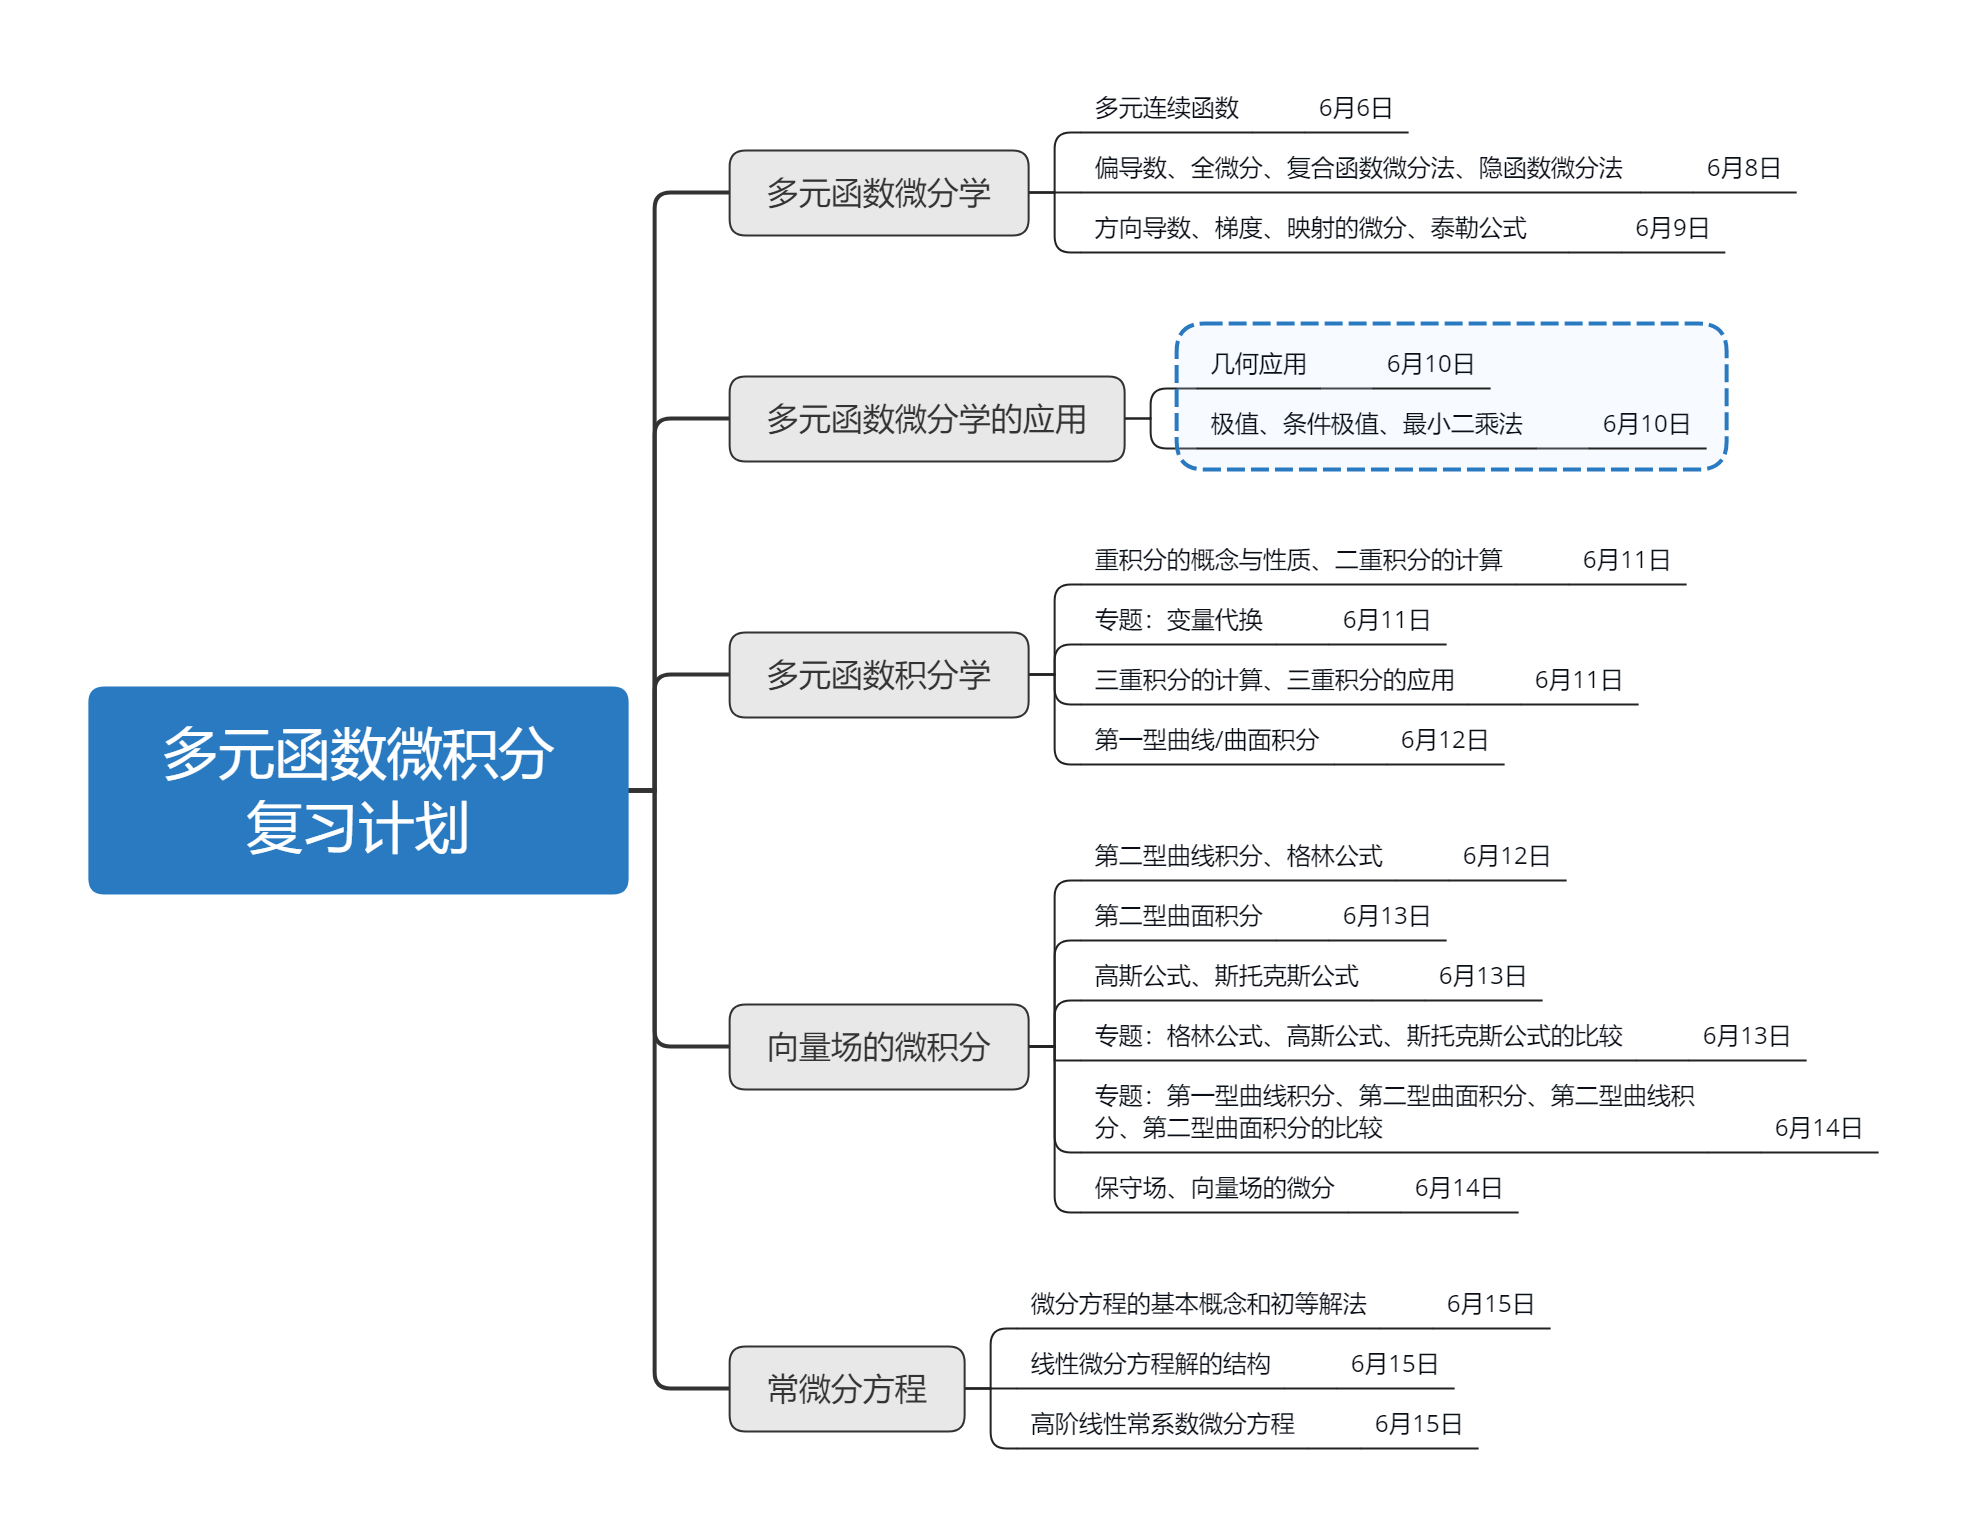
\includegraphics[height=0.5\textheight]{Figures20190610/plan.png}
\end{center}
\end{figure}
\subsection{知识结构}
\begin{figure}[H]
\begin{center}
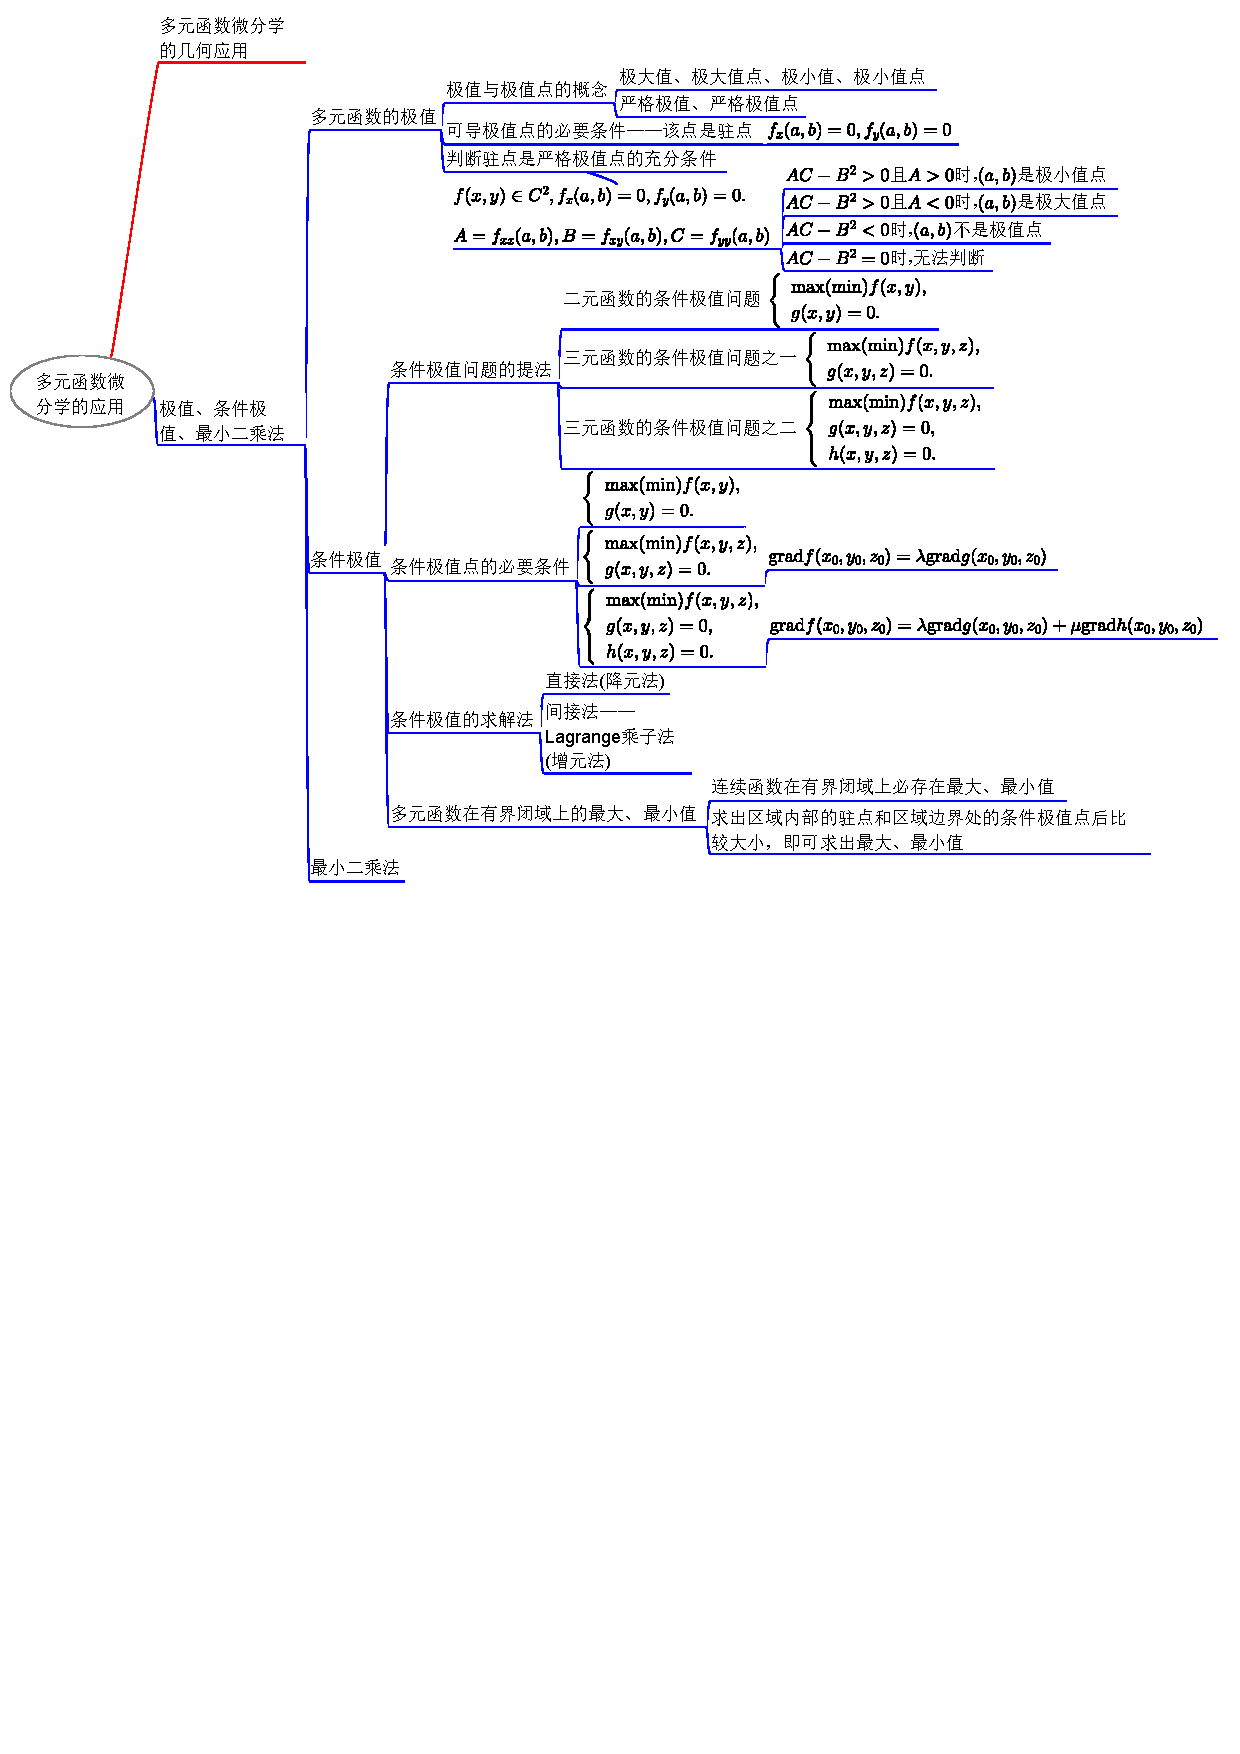
\includegraphics[height=0.9\textheight,angle=0]{20190610-1.pdf}
\end{center}
\end{figure}
\subsection{重要知识}
\subsection{习题分类与解题思路}
\begin{enumerate}
\item极值问题的求解思路:
\begin{enumerate}
\item[第一步]令函数的偏导数等于0,求出驻点;
\item[第二步]利用极值的充分条件判断驻点是否是极值,是最大值还是最小值;

【如习题11.3中的1.(1)/(2)/(3), 2., 3.】
\item[第三步]若用充分条件无法判断,则尝试其他办法求解.
\end{enumerate}
\item条件极值问题. 用Lagrange乘子法求解,须根据具体问题分析是否是极值. 主要有以下几种类型:
\begin{enumerate}
\item求解约束条件下的最值;

【如习题11.4中的1., 2., 3., 6.】
\item利用条件极值证明不等式.

【如习题11.4中的4., 5.】
\end{enumerate}
【这部分分析最值的方法大家可以做一个积累.】
\item有界闭区域上的最值问题. 只需求出驻点,比较大小,即可得到最大值和最小值. 不需用极值的充分条件判断.

【如习题11.4中的3.】
\end{enumerate}
\subsection{习题11.3解答}
\begin{enumerate}
\item求下列函数的极值,并判断是极大值还是极小值:\\
(1)$z=x^3+y^3-3xy$;\\
(2)$z=2xy-3x^3-2y^2+10$;\\
(3)$z=xy+\frac ax+\frac ay$.

解:(1)$\frac{\partial z}{\partial x}=3x^2-3y,\ \frac{\partial z}{\partial y}=3y^2-3x$,

令$\frac{\partial z}{\partial x}=0,\frac{\partial z}{\partial y}=0$得驻点$(0,0)$和$(1,1)$,

$\frac{\partial^2z}{\partial x^2}=6x,\ \frac{\partial^2z}{\partial x\partial y}=-3,\ \frac{\partial^2z}{\partial y^2}=6y$.

i)对于点$(0,0),\ A=\frac{\partial^2z(0,0)}{\partial x^2}=0,\ B=\frac{\partial^2z(0,0)}{\partial x\partial y}=-3,\ C=\frac{\partial^2z(0,0)}{\partial y^2}=0,\ AC-B^2=-9<0$,故$(0,0)$不是极值点;

ii)对于点$(1,1),\ A=\frac{\partial^2z(1,1)}{\partial x^2}=6,\ B=\frac{\partial^2z(1,1)}{\partial x\partial y}=-3,\ C=\frac{\partial^2z(1,1)}{\partial y^2}=6,\ AC-B^2=27>0,\ A>0$,故$(1,1)$是极小值点,极小值为$z(1,1)=-1$.

(2)$\frac{\partial z}{\partial x}=2y-9x^2,\ \frac{\partial z}{\partial y}=2x-4y$,

令$\frac{\partial z}{\partial x}=0,\frac{\partial z}{\partial y}=0$得驻点$(0,0)$和$(\frac19,\frac1{18})$,

$\frac{\partial^2z}{\partial x^2}=-18x,\ \frac{\partial^2z}{\partial x\partial y}=2,\ \frac{\partial^2z}{\partial y^2}=-4$.

i)对于点$(0,0),\ A=\frac{\partial^2z(0,0)}{\partial x^2}=0,\ B=\frac{\partial^2z(0,0)}{\partial x\partial y}=2,\ C=\frac{\partial^2z(0,0)}{\partial y^2}=-4,\ AC-B^2=-4<0$,故$(0,0)$不是极值点;

ii)对于点$(\frac19,\frac1{18}),\ A=\frac{\partial^2z(\frac19,\frac1{18})}{\partial x^2}=-2,\ B=\frac{\partial^2z(\frac19,\frac1{18})}{\partial x\partial y}=2,\ C=\frac{\partial^2z(\frac19,\frac1{18})}{\partial y^2}=-4,\ AC-B^2=4>0,\ A<0$,故$(\frac19,\frac1{18})$是极大值点,极大值为$z(\frac19,\frac1{18})=10\frac1{486}$.

(3)

(a)当$a\neq0$时,

$\frac{\partial z}{\partial x}=y+\frac{-a}{x^2},\ \frac{\partial z}{\partial y}=x+\frac{-a}{y^2}$,

令$\frac{\partial z}{\partial x}=0,\frac{\partial z}{\partial y}=0$得驻点$(\sqrt[3]a,\sqrt[3]a)$,

$\frac{\partial^2z}{\partial x^2}=\frac{2a}{x^3},\ \frac{\partial^2z}{\partial x\partial y}=1,\ \frac{\partial^2z}{\partial y^2}=\frac{2a}{y^3}$.

对于点$(\sqrt[3]a,\sqrt[3]a),\ A=\frac{\partial^2z(\sqrt[3]a,\sqrt[3]a)}{\partial x^2}=2,\ B=\frac{\partial^2z(\sqrt[3]a,\sqrt[3]a)}{\partial x\partial y}=1,\ C=\frac{\partial^2z(\sqrt[3]a,\sqrt[3]a)}{\partial y^2}=2,\ AC-B^2=3>0,\ A>0$,故点$(\sqrt[3]a,\sqrt[3]a)$是极小值点,极小值$z(\sqrt[3]a,\sqrt[3]a)=3\sqrt[3]{a^2}$.

(b)当$a=0$时$z(x,y)=xy$,

$\frac{\partial z}{\partial x}=y,\ \frac{\partial z}{\partial y}=x$,

令$\frac{\partial z}{\partial x}=0,\frac{\partial z}{\partial y}=0$得驻点$(0,0)$,

$\frac{\partial^2z}{\partial x^2}=0,\ \frac{\partial^2z}{\partial x\partial y}=1,\ \frac{\partial^2z}{\partial y^2}=0$.

对于点$(0,0),\ A=\frac{\partial^2z(0,0)}{\partial x^2}=0,\ B=\frac{\partial^2z(0,0)}{\partial x\partial y}=1,\ C=\frac{\partial^2z(0,0)}{\partial y^2}=0,\ AC-B^2=-1<0$,故点$(0,0)$不是是极值点.

\item设函数$z=z(x,y)$由方程$4x^2+2y^2+3z^2-4xy-2yz-8=0$确定,求$z=z(x,y)$的极值点.

解:方程$4x^2+2y^2+3z^2-4xy-2yz-8=0$两边分别对$x,y$求偏导:
\begin{subequations}
\begin{align}
&8x+6z\frac{\partial z}{\partial x}-4y-2y\frac{\partial z}{\partial x}=0,\label{2-1a}\\
&4y+6z\frac{\partial z}{\partial y}-4x-2z-2y\frac{\partial z}{\partial y}=0.\label{2-1b}
\end{align}
\end{subequations}
在以上两式中令$\frac{\partial z}{\partial x}=0,\frac{\partial z}{\partial y}=0$得$\begin{cases}
8x-4y=0,\\
4y-4x-2z=0,
\end{cases}$与$4x^2+2y^2+3z^2-4xy-2yz-8=0$联立,得驻点$(1,2)$和$(-1,-2)$,且$z(1,2)=2,\ z(-1,-2)=-2$,

方程~(\ref{2-1a})两边分别对$x,y$求偏导:
\begin{subequations}
\begin{align}
&8+6(\frac{\partial z}{\partial x})^2+6z\frac{\partial^2z}{\partial x^2}-2y\frac{\partial^2z}{\partial x^2}=0,\label{2-2a}\\
&6\frac{\partial z}{\partial y}\frac{\partial z}{\partial x}+6z\frac{\partial^2z}{\partial y\partial x}-4-2\frac{\partial z}{\partial x}-2y\frac{\partial^2z}{\partial y\partial x}=0,\label{2-2b}
\end{align}
\end{subequations}
方程~(\ref{2-1b})两边分别对$y$求偏导:
\begin{equation}\label{3}
4+6(\frac{\partial z}{\partial y})^2+6z\frac{\partial^2z}{\partial y^2}-2\frac{\partial z}{\partial y}-2\frac{\partial z}{\partial y}-2y\frac{\partial^2z}{\partial y^2}=0.
\end{equation}
i)将$x=1,y=2,z=2,\frac{\partial z}{\partial x}=0,\frac{\partial z}{\partial y}=0$代入方程~(\ref{2-2a})、~(\ref{2-2b})和~(\ref{3}),令$A=\frac{\partial^2z(1,2)}{\partial x^2},B=\frac{\partial^2z(1,2)}{\partial x\partial y},C=\frac{\partial^2z(1,2)}{\partial y^2}$得
\[\begin{split}
8+12A-4A=0,\\
12B-4-4B=0,\\
4+12C-4C=0,
\end{split}\]
解得$A=-1,B=\frac12,C=-\frac12,\ AC-B^2=\frac12>0,\ A=-1<0$,故$(1,2)$是函数$z=z(x,y)$的极大值点.

ii)将$x=-1,y=-2,z=-2,\frac{\partial z}{\partial x}=0,\frac{\partial z}{\partial y}=0$代入方程~(\ref{2-2a})、~(\ref{2-2b})和~(\ref{3}),令$A=\frac{\partial^2z(-1,-2)}{\partial x^2},B=\frac{\partial^2z(-1,-2)}{\partial x\partial y},C=\frac{\partial^2z(-1,-2)}{\partial y^2}$得
\[\begin{split}
8-12A+4A=0,\\
-12B-4+4B=0,\\
4-12C+4C=0,
\end{split}\]解得$A=1,B=-\frac12,C=\frac12,\ AC-B^2=\frac12>0,\ A=1>0$,故$(-1,-2)$是函数$z=z(x,y)$的极小值点.

\item试证函数$z=(1+\mathrm e^y)\cos x-y\mathrm e^y$有无穷多个极大值而无极小值.

证明:$\frac{\partial z}{\partial x}=-(1+\mathrm e^y)\sin x,\ \frac{\partial z}{\partial y}=(\cos x-1-y)\mathrm e^y$,

令$\frac{\partial z}{\partial x}=0,\frac{\partial z}{\partial y}=0$得驻点$(k\pi,(-1)^k-1),k\in\mathbb Z$,

$\frac{\partial^2z}{\partial x^2}=-(1+\mathrm e^y)\cos x,\ \frac{\partial^2z}{\partial x\partial y}=-\mathrm e^y\sin x,\ \frac{\partial^2z}{\partial y^2}=(\cos x-1-y-1)\mathrm e^y=(\cos x-y-2)\mathrm e^y$.

在驻点$(k\pi,(-1)^k-1),k\in\mathbb Z$处,

$A=\frac{\partial^2z(k\pi,(-1)^k-1)}{\partial x^2}=-[1+\mathrm e^{(-1)^k-1}]\cos k\pi=-[1+\mathrm e^{(-1)^k-1}](-1)^k$,

$B=\frac{\partial^2z(k\pi,(-1)^k-1)}{\partial x\partial y}=-\mathrm e^{(-1)^k-1}\sin k\pi=0$,

$C=\frac{\partial^2z(k\pi,(-1)^k-1)}{\partial y^2}=[\cos k\pi-(-1)^k+1-2]\mathrm e^{(-1)^k-1}=-\mathrm e^{(-1)^k-1}$,

$AC-B^2=\mathrm e^{(-1)^k-1}[1+\mathrm e^{(-1)^k-1}](-1)^k=\begin{cases}
-\mathrm e^{-2}(1+\mathrm e^{-2})<0,&k=2n-1,\\
2>0,&k=2n,
\end{cases}n\in\mathbb Z$,

故当$k$为奇数时$(k\pi,(-1)^k-1)$不是极值点;当$k$为偶数时,$A=-2<0$,故$(k\pi,(-1)^k-1)$是极大值点.

因此函数$z=(1+\mathrm e^y)\cos x-y\mathrm e^y$有无穷多个极大值而无极小值.
\end{enumerate}
\subsection{习题11.4解答}
\begin{enumerate}
\item在抛物线$y^2=4x$上求一点,使其到点$(2,8)$的距离最短.

解:抛物线$y^2=4x$的点与点$(2,8)$的距离的平方
\[d^2=(x-2)^2+(y-8)^2=(\frac14y^2-2)^2+(y-8)^2,\]
$\therefore$
\[\frac{\mathrm dd^2}{\mathrm dy}=2(\frac14y^2-2)\frac12y+2(y-8)=\frac14y^3-2y+2y-16=\frac14y^3-16,\]
令$\frac{\mathrm dd^2}{\mathrm dy}=0$得$y=4$,此时$x=4$,则抛物线$y^2=4x$上到点$(2,8)$的距离最短的点为$(4,4)$.

【关于最值的分析:】在抛物线$y^2=4x$上当$y=8$时$x=4>2$,故点$(2,8)$在抛物线开口外部,则以点$(2,8)$为圆心作圆与抛物线相切,这样的圆只有一个,其半径为抛物线上的到点$(2,8)$距离的最小值. 该最小值也是极小值,满足导数为零的条件,现在满足导数为零条件的点只有一个,则该点就是最小值点.
\item在椭球面$\frac{x^2}{a^2}+\frac{y^2}{b^2}+\frac{z^2}{c^2}=1$内嵌入一长方体,使其体积最大,并求此最大值.

解:设该长方体在第一象限内的顶点为$(x,y,z),x>0,y>0,z>0$,问题转化为条件极值问题$\begin{cases}
\max\{8xyz\},\\
s.t.\ \frac{x^2}{a^2}+\frac{y^2}{b^2}+\frac{z^2}{c^2}=1.
\end{cases}$

令$L(x,y,z,\lambda)=8xyz+\lambda(\frac{x^2}{a^2}+\frac{y^2}{b^2}+\frac{z^2}{c^2}-1)$,\\
由$\begin{cases}
\frac{\partial L}{\partial x}=8yz-2\lambda\frac x{a^2}=0,\\
\frac{\partial L}{\partial y}=8xz-2\lambda\frac y{b^2}=0,\\
\frac{\partial L}{\partial z}=8xy-2\lambda\frac z{c^2}=0,\\
\frac{\partial L}{\partial\lambda}=\frac{x^2}{a^2}+\frac{y^2}{b^2}+\frac{z^2}{c^2}-1=0,
\end{cases}$得$(x,y,z)=(\frac a{\sqrt3},\frac b{\sqrt3},\frac c{\sqrt3})$,

故当该长方体在第一卦限内的顶点为$(\frac a{\sqrt3},\frac b{\sqrt3},\frac c{\sqrt3})$时,体积最大,最大值为$V_{\max}=\frac8{3\sqrt3}abc$.

【关于最值的分析:】在第一象限内椭球面$\frac{x^2}{a^2}+\frac{y^2}{b^2}+\frac{z^2}{c^2}=1,x>0,y>0,z>0$的边界上,长方体的体积为$0$,在第一象限的椭球面内部,$0<V=8xyz<8abc$,$V$有上界,故有上确界,易知此时的上确界是$V=8xyz$的最大值. 最大值也是极值,满足极值存在的必要条件,现在根据极值存在的必要条件只求出了一个点,故该点是唯一的最值点,故是最大值点. 

\item求$f(x,y)=x^2+y^2-x-y$在$B=\Set{(x,y)}{x^2+y^2\leq1}$上的最大值与最小值.

解:由$\begin{cases}
\frac{\partial f}{\partial x}=2x-1=0,\\
\frac{\partial f}{\partial y}=2y-1=0,
\end{cases}$得$(x,y)=(\frac12,\frac12)$,

令$L(x,y,\lambda)=x^2+y^2-x-y+\lambda(x^2+y^2-1)$,由$\begin{cases}
\frac{\partial L}{\partial x}=2x-1+2\lambda x=0,\\
\frac{\partial L}{\partial y}=2y-1+2\lambda y=0,\\
\frac{\partial L}{\partial\lambda}=x^2+y^2-1=0,
\end{cases}$\\
得$(x,y)=(\pm\frac{\sqrt2}2,\pm\frac{\sqrt2}2)$,

$\because f(\frac12,\frac12)=-\frac12,f(\frac{\sqrt2}2,\frac{\sqrt2}2)=1-\sqrt2,f(-\frac{\sqrt2}2,-\frac{\sqrt2}2)=1+\sqrt2$,

$\therefore f(x,y)$在$B$上的最大值为$1+\sqrt2$,最小值为$-\frac12$.

\item求函数$f(x,y,z)=x^2y^2z^2$在约束条件$x^2+y^2+z^2=c^2$下的最大值,并证明不等式
\[
\sqrt[3]{x^2y^2z^2}\leq\frac{x^2+y^2+z^2}3.
\]
解:条件极值问题$\begin{cases}
\max\{x^2y^2z^2\},\\
s.t.\ x^2+y^2+z^2=c^2,
\end{cases}$等价为在$u>0,v>0,w>0$时的条件极值问题$\begin{cases}
\max\{uvw\},\\
s.t.\ u+v+w=c^2,
\end{cases}$

令$L(u,v,w,\lambda)=uvw+\lambda(u+v+w-c^2)$,由$\begin{cases}
\frac{\partial L}{\partial u}=vw+\lambda=0,\\
\frac{\partial L}{\partial v}=uw+\lambda=0,\\
\frac{\partial L}{\partial w}=uv+\lambda=0,\\
\frac{\partial L}{\partial\lambda}=u+v+w-c^2=0,
\end{cases}$\\
得$(u,v,w)=(\frac{c^2}3,\frac{c^2}3,\frac{c^2}3)$,则所求最大值为$f(\frac{c}{\sqrt3},\frac{c}{\sqrt3},\frac{c}{\sqrt3})=\frac{c^6}{27}$(不妨设$c>0$).

对任意实数$x,y,z$,取$c^2=x^2+y^2+z^2$,则
\[x^2y^2z^2\leq\frac{c^6}{27}=\frac{x^2+y^2+z^2}{27},\]
即
\[\sqrt[3]{x^2y^2z^2}\leq\frac{x^2+y^2+z^2}3.\]

【关于最值的分析:】在第一象限的平面$u+v+w=c^2,u>0,v>0,w>0$上,$0<uvw<c^6$,$uvw$有上界,故有上确界,易知该上确界也是最大值. 最大值也是极大值,满足极值存在的必要条件,现在根据该必要条件只求出了一个点,则该点就是最大值点.

\item设$x,y$为任意正数,求证
\[\frac{x^n+y^n}2\geqslant(\frac{x+y}2)^n.\]
(提示:在约束条件$x+y=a$下,求$z=\frac12(x^n+y^n)$的极值.)

证明:当$n=1$时,$\frac{x^n+y^n}2\geqslant(\frac{x+y}2)^n$显然成立;

当$n\geqslant2$时,对于任意正数$x,y$,求解条件极值问题$\begin{cases}
\min\{\frac12(x^n+y^n)\},\\
s.t.\ x+y=a,
\end{cases}$\\
令$L(x,y,\lambda)=\frac12(x^n+y^n)+\lambda(x+y-a)$,\\
由$\begin{cases}
\frac{\partial L}{\partial x}=\frac n2x^{n-1}+\lambda=0,\\
\frac{\partial L}{\partial y}=\frac n2y^{n-1}+\lambda=0,\\
\frac{\partial L}{\partial\lambda}=x+y-a=0,
\end{cases}(*)$得$(x,y)=(\frac a2,\frac a2)$,\\
故$z(x,y)=\frac12(x^n+y^n)\geqslant z(\frac a2,\frac a2)=(\frac a2)^n$.

对于任意正数$x,y$,取$a=x+y$,则
\[
\frac{x^n+y^n}2\geqslant(\frac a2)^n=(\frac{x+y}2)^n.
\]

【注意:】(1)这里$n$的范围应为正整数;(2)当$n=1$时,线段$x+y=1,x>0,y>0$上的任意一点均满足方程组$(*)$,可能的极值点不唯一,故应分成$n=1$和$n\geqslant2$两种情况考虑. 这也和$n=1$时在线段$x+y=1,x>0,y>0$上$\frac12(x^n+y^n)=\frac12(x+y)=\frac12a$为常数一致.

【关于最值的分析:】当$n=1$时,在线段$x+y=1,x>0,y>0$上$\frac12(x+y)=\frac 12$;

当$n=2$时,$\frac12(x^2+y^2)$在线段$x+y=1,x\geqslant0,y\geqslant0$的两端点处等于$\frac12$,在该线段的内部因$0<x<1,0<y<1$,故$\frac12(x^2+y^2)<\frac12(x+y)=\frac12$;

同理,当$n=3$时,$\frac12(x^3+y^3)$在线段$x+y=1,x\geqslant0,y\geqslant0$的两端点处等于$\frac12$,在该线段的内部因$0<x<1,0<y<1$,故$\frac12(x^3+y^3)<\frac12(x^2+y^2)<\frac12(x+y)=\frac12$.

故$\forall(x,y)\in\Set{(x,y)}{x+y=1,x>0,y>0},\frac12(x^n+y^n)<\cdots<\frac12(x^3+y^3)<\frac12(x^2+y^2)<\frac12(x+y)=\frac12$,因为在线段$x+y=1,x>0,y>0$上$\frac12(x^2+y^2)=\frac12[x^2+(1-x)^2]=x(x-1)+\frac12$,为一开口向上的抛物线,最高的两点的值为$\frac12$,故当$n\geqslant2$时$\frac12(x^n+y^n)$在线段$x+y=1,x>0,y>0$上均为下凸函数,则$\frac12[(\frac xa)^n+(\frac ya)^n]=\frac1{2a^n}(x^n+y^n)$在线段$\frac xa+\frac ya=1,x>0,y>0$上也为下凸函数,则$\frac12(x^n+y^n)$在线段$\frac xa+\frac ya=1,x>0,y>0$即$x+y=a,x>0,y>0$上也为下凸函数,故必有最小值. 最小值也是极小值,满足极值的必要条件,因满足极值必要条件的点只有一个,故该点就是最小值点.

\item求曲面$S_1:z=x^2+y^2$与$S_2:x+y+z=1$的交线上到原点的距离最大与最小的点.

解:曲面$S_1$与$S_2$的交线上的点$(x,y,z)$到原点的距离$r(x,y,z)=\sqrt{x^2+y^2+z^2}$,问题是求解条件极值$\begin{cases}
\max(\min)\{\sqrt{x^2+y^2+z^2}\},\\
s.t.\quad z=x^2+y^2,\\
\ \ \ \ \quad x+y+z=1,
\end{cases}$可化为条件极值问题$\begin{cases}
\max(\min)\{x^2+y^2+z^2\},\\
s.t.\quad z=x^2+y^2,\\
\ \ \ \ \quad x+y+z=1,
\end{cases}$\\
令$L(x,y,z,\lambda)=x^2+y^2+z^2+\lambda(x^2+y^2-z)+\mu(x+y+z-1)$,\\
由$\begin{cases}
\frac{\partial L}{\partial x}=2x+2\lambda x+\mu=0,\\
\frac{\partial L}{\partial y}=2y+2\lambda y+\mu=0,\\
\frac{\partial L}{\partial z}=2z-\lambda+\mu=0,\\
\frac{\partial L}{\partial\lambda}=x^2+y^2-z=0,\\
\frac{\partial L}{\partial\mu}=x+y+z-1=0,
\end{cases}$得$(x,y,z)=(\frac{\pm\sqrt3-1}2,\frac{\pm\sqrt3-1}2,2\mp\sqrt3)$,

由$r(\frac{\sqrt3-1}2,\frac{\sqrt3-1}2,2-\sqrt3)=\sqrt{9-5\sqrt3},f(-\frac{\sqrt3+1}2,-\frac{\sqrt3+1}2,2+\sqrt3)=\sqrt{9+5\sqrt3}$得曲面$S_1$与$S_2$的交线上到原点距离最大的点为$(-\frac{\sqrt3+1}2,-\frac{\sqrt3+1}2,2+\sqrt3)$,距离最小的点为$(\frac{\sqrt3-1}2,\frac{\sqrt3-1}2,2-\sqrt3)$.

【关于最值的分析:】旋转抛物面$S_1$与平面$S_2$的交线是一条光滑封闭曲线,在该曲线上必有到原点距离最大和最小的点,这两点均是极值点,满足极值的必要条件,现在根据极值的必要条件只求出两个点,故这两个点一个是最大值点,一个是最小值点.

\item将长为$l$的线段分成三份,分别围成圆、正方形和正三角形,问如何分割才能使他们的面积之和最小,并求此最小值.

解:设$x,y,z$分别是围成圆、正方形和正三角形的线段长度,问题是求解条件极值\\
$\begin{cases}
\min\{f(x,y,z)=\pi(\frac x{2\pi})^2+(\frac y4)^2+\frac{\sqrt3}4(\frac z3)^2\},\\
s.t.\quad x+y+z=l,
\end{cases}$\\
令$L(x,y,z,\lambda)=\pi(\frac x{2\pi})^2+(\frac y4)^2+\frac{\sqrt3}4(\frac z3)^2+\lambda(x+y+z-l)$,\\
由$\begin{cases}
\frac{\partial L}{\partial x}=\frac x{2\pi}+\lambda=0,\\
\frac{\partial L}{\partial y}=\frac18y+\lambda=0,\\
\frac{\partial L}{\partial z}=\frac{\sqrt3}{18}z+\lambda=0,\\
\frac{\partial L}{\partial\lambda}=x+y+z-l=0,
\end{cases}$得$(x,y,z)=(\frac{\pi l}{\pi+4+3\sqrt3},\frac{4l}{\pi+4+3\sqrt3},\frac{3\sqrt3l}{\pi+4+3\sqrt3})$,

故当围成圆、正方形和三角形的三条线段的长度分别为$\frac{\pi l}{\pi+4+3\sqrt3},\frac{4l}{\pi+4+3\sqrt3},\frac{3\sqrt3l}{\pi+4+3\sqrt3}$时,它们的面积和最小,最小值为$f(\frac{\pi l}{\pi+4+3\sqrt3},\frac{4l}{\pi+4+3\sqrt3},\frac{3\sqrt3l}{\pi+4+3\sqrt3})=\frac{(\pi+4+3\sqrt3)l^2}{4(\pi+4+3\sqrt3)^2}$.

【关于最值的分析:】当椭球面$S=\pi(\frac x{2\pi})^2+(\frac y4)^2+\frac{\sqrt3}4(\frac z3)^2\}$与第一象限的平面$x+y+z=l$相切时,$S$为最小,切点位于第一象限,故满足条件的最小值点存在,最小值点也是极小值点,满足极值的必要条件,现在根据极值的必要条件只求出了一个点,故该点就是最小值点. 
\end{enumerate}
\subsection{第11章补充题解答}
\begin{enumerate}
\item确定正数$a$,使得椭球面$x^2+\frac{y^2}4+\frac{z^2}9=a^2$与平面$x-2y+3z=100$相切.

解:方法1:平面$x-2y+3z=100$的法向量$\bm n_0=(1,-2,3)$,

设切点为$(x_0,y_0,z_0)$,椭球面在切点处的法向量$\bm n=(2x,\frac12y,\frac29z)\big|_{(x_0,y_0,z_0)}=(2x_0,\frac12y_0,\frac29z_0)$,

由$\bm n\parallel\bm n_0$知$(2x_0,\frac12y_0,\frac29z_0)=\lambda(1,-2,3)$,又知切点$(x_0,y_0,z_0)$应满足直线方程$x_0-2y_0+3z_0=100$,可得$\lambda=\frac{100}{49}$,

%则切点为$(x_0,y_0,z_0)=(\frac{50}{49},-\frac{400}{49},\frac{1350}{49})$,
故$a^2=x_0^2+\frac{y_0^2}4+\frac{z_0^2}9=\frac{\lambda^2}4+4\lambda^2+\frac{81}4\lambda^2=\frac{98}4(\frac{100}{49})^2=\frac{5000}{49},\ a=\frac{50}7\sqrt2$.

方法2:如限定椭球面$x^2+\frac{y^2}4+\frac{z^2}9=a^2$与平面$x-2y+3z=100$相交或相切,则当相切时$a^2$最小,因此问题等价于条件极值问题$\begin{cases}
\min{x^2+\frac{y^2}4+\frac{z^2}9},\\
s.t.\ x-2y+3z=100,
\end{cases}$

令$L(x,y,z,\lambda)=x^2+\frac{y^2}4+\frac{z^2}9+\lambda(x-2y+3z-100)$,

由$\begin{cases}
\frac{\partial L}{\partial x}=2x+\lambda=0,\\
\frac{\partial L}{\partial y}=\frac12y-2\lambda=0,\\
\frac{\partial L}{\partial z}=\frac29z+3\lambda=0,\\
\frac{\partial L}{\partial\lambda}=x-2y+3z-100=0,
\end{cases}$得$(x,y,z)=-\frac{100}{49}(-\frac12,4,-\frac{27}2)$,

故所求最小值为$a^2=x^2+\frac{y^2}4+\frac{z^2}9=(\frac14+4+\frac{81}4)(\frac{100}{49})^2=\frac{5000}{49},\ a=\frac{50}7\sqrt2$.

\item设$f(x,y)$在全平面内可微,并且当$x^2+y^2\rightarrow+\infty$时,满足条件
\[
\frac{|f(x,y)|}{\sqrt{x^2+y^2}}\rightarrow+\infty.
\]
求证:对于任意向量$\bm v=(v_1,v_2)$,存在点$M(x_0,y_0)$,使得$\mathrm{grad}f(x_0,y_0)=\bm v$.

证明:$\because\frac{|f(x,y)|}{\sqrt{x^2+y^2}}\rightarrow+\infty,x^2+y^2\rightarrow+\infty$,

$\therefore|f(x,y)|=\frac{|f(x,y)|}{\sqrt{x^2+y^2}}\sqrt{x^2+y^2}\rightarrow+\infty,x^2+y^2\rightarrow+\infty$,

下面证明:当$x^2+y^2\rightarrow+\infty$时,或者$f(x,y)\rightarrow+\infty$或者$f(x,y)\rightarrow-\infty$.

$\because|f(x,y)|\rightarrow+\infty,x^2+y^2\rightarrow+\infty$,

$\therefore\exists R>0,s.t.$当$x^2+y^2>R^2$时,$|f(x,y)|>1$,

假设当$x^2+y^2\rightarrow+\infty$时,既不是$f(x,y)\rightarrow+\infty$,也不是$f(x,y)\rightarrow-\infty$. 则必存在两点$M_1(x_1,y_1),M_2(x_2,y_2)$,满足$x_1^2+y_1^2>R^2,x_2^2+y_2^2>R^2$,且$f(x_1,y_1)<0,f(x_2,y_2)>0$. 以点$M_1(x_1,y_1),M_2(x_2,y_2)$分别为起点和终点做一条完全位于圆域$\Set{(x,y)}{x^2+y^2\leq R^2}$之外的连续曲线$L$,在该曲线上$f(x,y)$为一元连续函数,根据零点定理$\exists M(\xi,\eta)\in L,s.t.f(\xi,\eta)=0$. 但在曲线$L$上$x^2+y^2>R^2$,故$\forall(x,y)\in L,|f(x,y)|>1$,与$\exists M(\xi,\eta)\in L,s.t.f(\xi,\eta)=0$矛盾. 故假设不成立. 

所以当$x^2+y^2\rightarrow+\infty$时,或者$f(x,y)\rightarrow+\infty$或者$f(x,y)\rightarrow-\infty$.

对于任意向量$\bm v=(v_1,v_2)$,

$\because|\frac{v_1x+v_2y}{\sqrt{x^2+y^2}}|\leq\frac{|v_1||x|+|v_2||y|}{\sqrt{x^2+y^2}}\leq\frac{|v_1||x|}{|x|}+\frac{|v_1||y|}{|y|}=|v_1|+|v_2|$,

$\therefore\frac{|f(x,y)-(v_1x+v_2y)|}{\sqrt{x^2+y^2}}\geq\frac{|f(x,y)|}{\sqrt{x^2+y^2}}-|\frac{v_1x+v_2y}{\sqrt{x^2+y^2}}|\geq\frac{|f(x,y)|}{\sqrt{x^2+y^2}}-(|v_1|+|v_2|)$,

$\because\frac{|f(x,y)|}{\sqrt{x^2+y^2}}\rightarrow+\infty,x^2+y^2\rightarrow+\infty$,

$\therefore\frac{|f(x,y)-(v_1x+v_2y)|}{\sqrt{x^2+y^2}}\rightarrow+\infty,x^2+y^2\rightarrow+\infty$,

$\therefore$与证明当$x^2+y^2\rightarrow+\infty$时,或者$f(x,y)\rightarrow+\infty$或者$f(x,y)\rightarrow-\infty$同理,当$x^2+y^2\rightarrow+\infty$时,或者$f(x,y)-(v_1x+v_2y)\rightarrow+\infty$或者$f(x,y)-(v_1x+v_2y)\rightarrow-\infty$,

不妨设当$x^2+y^2\rightarrow+\infty$时,$f(x,y)-(v_1x+v_2y)\rightarrow+\infty$,

根据第10章补充题第1题的结论,$\exists(x_0,y_0),s.t.g(x,y)=f(x,y)-(v_1x+v_2y)\geq g(x_0,y_0)$. 

则在点$(x_0,y_0)$处$\frac{\partial g(x_0,y_0)}{\partial x}=\frac{\partial f(x_0,y_0)}{\partial x}-v_1=0,\frac{\partial g(x_0,y_0)}{\partial y}=\frac{\partial f(x_0,y_0)}{\partial y}-v_2=0$,即$\mathrm{grad}f(x_0,y_0)=(\frac{\partial f(x_0,y_0)}{\partial x},\frac{\partial f(x_0,y_0)}{\partial y})=(v_1,v_2)=\bm v$,

所以对于任意向量$\bm v=(v_1,v_2)$,存在点$M(x_0,y_0)$,使得$\mathrm{grad}f(x_0,y_0)=\bm v$.

\item设$f(x,y)=3x^4-4x^2y+y^2$. 求证:若限制在过原点的每条直线上,$f(x,y)$在原点达到极小值. 但是原点不是$f(x,y)$的极小值.

证明:(1)$f(0,y)=y^2$在$y=0$处达到极小值,即在直线$x=0$上$f(x,y)$在原点处达到极小值.

(2)记$g(x)=f(x,kx)=3x^4-4kx^3+k^2x^2$,

则$g'(x)=12x^3-12kx^2+2k^2x,\ g''(x)=36x^2-24kx+2k^2$,

i)当$k\neq0$时,$g'(0)=0,\ g''(0)=2k^2>0$,$g(x)$在点$x=0$处取得极小值;

ii)当$k=0$时,$g(x)=3x^4$,$g(x)$在点$x=0$处取得极小值.

故在直线$y=kx$上$f(x,y)$在原点处达到极小值.

所以在过原点的每条直线上,$f(x,y)$在原点达到极小值.

$\because\frac{\partial f}{\partial x}=12x^3-8xy,\ \frac{\partial f}{\partial y}=-4x^2+2y$,

$\frac{\partial^2f}{\partial x^2}=36x^2-8y,\ \frac{\partial^2f}{\partial x\partial y}=-8x,\ \frac{\partial^2f}{\partial y^2}=2$,

$\therefore$在原点$(0,0)$处$\frac{\partial f(0,0)}{\partial x}=0,\ \frac{\partial f(0,0)}{\partial y}=0$,

且$A=\frac{\partial^2f(0,0)}{\partial x^2}=0,\ B=\frac{\partial^2f(0,0)}{\partial x\partial y}=0,\ C=\frac{\partial^2f(0,0)}{\partial y^2}=2,\ AC-B^2=0$,

又$\because f(x,2x^2)=3x^4-8x^4+4x^4=-x^4$在$x=0$处取得极大值,即在抛物线$y=2x^2$上$f(x,y)$在原点处取得极大值,故原点不是$f(x,y)$的极小值.
\end{enumerate}
\end{document}